\newtheorem{PolicyDef}{Definition}


\chapter{Integration with the Barbeque Run-Time Resource Manager}
\label{cap:integration}
In this chapter we present the integration of the \texttt{mig} framework
with the Barbeque Run-Time Resource Manager \cite{bellasi2012rtrm},
shorten BarbequeRTRM. The BarbequeRTRM is a framework to manage the resources
of both heterogeneous and homogeneous systems at run-time. The extension of BarbequeRTRM that adds the capability
to manage distributed systems is described. Subsequently, an example of exploitation of
\texttt{mig} with a policy that takes into account
resources located into remote systems is presented.

\section{The BarbequeRTRM - Open MPI interface}
Following the implementation of other resource managers in Open MPI, we decided
to implement a socket client-server paradigm in order to interface the BarbequeRTRM to the Open MPI runtime and vice versa.

\subsection{The \texttt{bbque-mpirun} launcher}

As a first step, we introduced in the BarbequeRTRM a custom MPI application
launcher, \texttt{bbque-mpirun}, acting as a wrapper of the well-known
\texttt{mpirun} command commonly available in every MPI implementation. This
is order to enable the possibility of controlling the execution flow of MPI processes, by the BarbequeRTRM. 
The launcher exploits the already available BarbequeRTRM 
\textbf{Run-Time Library (RTLib)}
API to communicate with the BarbequeRTRM.

When invoked very first step of the \texttt{bbque-mpirun} launcher is
to open a socket listening onto a specific TCP port and the spawning
an instance of underlying \texttt{mpirun} launcher. When the \texttt{ras}
component of BarbequeRTRM is selected, recognizing a previously set environment variable and loaded, it connects
to the open socket of \texttt{bbque-mpirun}. At this point \texttt{mpirun}
sends the nodes request (specifically the number of \emph{slots}, i.e. the
total number of processes to be spawned in each node). \texttt{bbque-mpirun}
receives the request and it sends through to the
BarbequeRTRM. Subsequently, the resource manager can select an available set
of computing nodes, according to a policy, and send it to the  \texttt{bbque-mpirun} as reply,
that in turn is forwarded to \texttt{mpirun}.

It is worth to specify that \texttt{bbque-mpirun} is multi-threaded piece
of software implemented in C++, which operates as shown in the UML Sequence Diagram in Figure \ref{fig:cap5-sequencempirun}:
\begin{itemize}
\item The main thread follows the normal BarbequeRTRM applications
      execution, exchanging data like performance measurements and
      reconfiguration (not yet implemented). In case the BarbequeRTRM
      changes the allocation, it is in charge of notifying it to the
      \texttt{mpirun} instance;

\item A second thread is waiting on the TCP socket connected with
      \texttt{mpirun}. Currently only diagnostic messages for migration
      are sent over that channel. This thread is implemented in the
      \texttt{CommandManager} class.

\item A third thread is in charge to check the abnormal termination of
      \texttt{mpirun}
      process before the establishment of the socket connection. This thread
      is implemented in the \texttt{ProcessChecker} class.
\end{itemize}

\begin{figure}[t]
    \centerline 
{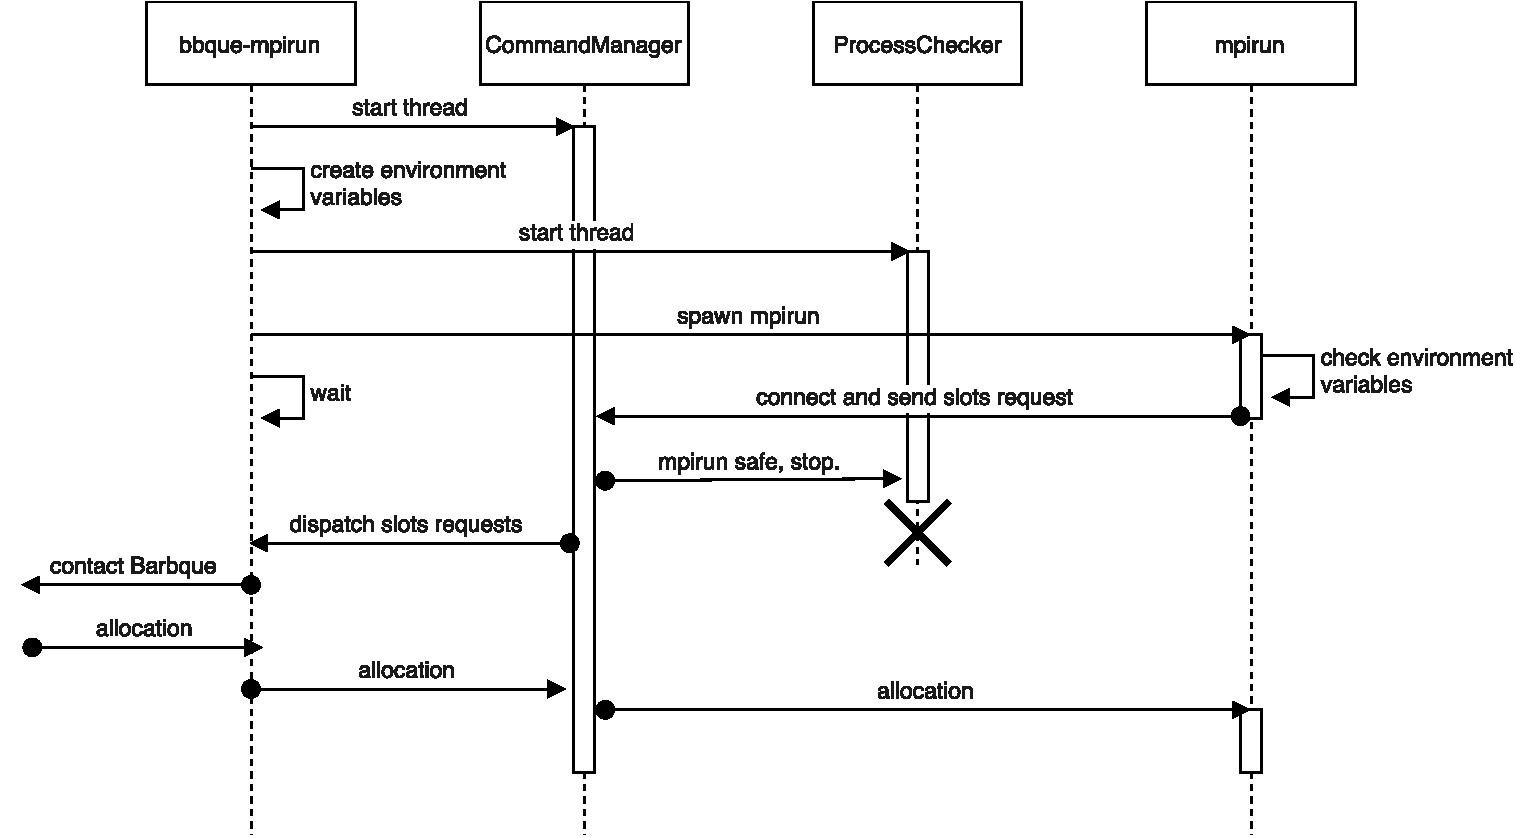
\includegraphics[scale=0.5]{img/cap5-sequencempirun.pdf}}
    \caption[UML Sequence Diagram of \texttt{bbque-mpirun}]{The UML Sequence Diagram of the \texttt{bbque-mpirun} tool.}
    \label{fig:cap5-sequencempirun}
\end{figure}

As already introduced, \texttt{bbque-mpirun} may be considered as a wrapper of
\texttt{mpirun} command, that establishes a link between BarbequeRTRM and the
Open MPI framework. This approach is similar to the one adopted by \emph{SLURM}
resource manager.

\section{Towards the BarbequeRTRM distributed version}
BarbequeRTRM was designed  to be a run-time resource manager targeting
single node systems. In parallel with \texttt{mig} development, this work is
the first step towards the development of a distributed
version of the BarbequeRTRM.

In order to correctly manage MPI applications and to
select an appropriate allocation over the distributed nodes, the BarbequeRTRM
has to know how many nodes are in the systems and how they are characterized.

Calculate the optimal processes allocation over the nodes and future
rescheduling - thus the evaluation of a favorable migration - are duties of an
appropriate policy, which is introduced in the next section.

In BarbequeRTRM the available resource retrieval and the fulfillment of a
scheduling are a task of the \texttt{PlatformProxy} component.
The \linebreak \texttt{PlatformProxy}
interface was previously implemented by a system-specific subclass, e.g.
the Linux and OpenCL implementations.
We have redesigned the 
\texttt{PlatformProxy} in a more hierarchical fashion, adding a \linebreak 
\texttt{LocalPlatformProxy} and a
\texttt{RemotePlatformProxy} component. The former has the duty of providing a
transparent
layer to the resources, like local CPU cores and OpenCL devices, while the latter is in charge of
communicating with available remote BarbequeRTRM instances, if any. 
The conceptual diagram of the BarbequeRTRM components that allows to
work in a distributed environment is shown in Figure \ref{fig:cap5-conc-diag}.
As shown 


Since we are in the early stages of the design of a distributed version of
BarbequeRTRM, the described design may change in next months. Furthermore, the
information needed by the scheduling policy - subsequently passed to
\texttt{bbque-mpirun} - is currently retrieved via
\texttt{RemotePlatformProxy} that in turn reads a static XML file,
containing the information of remote nodes.


The platform manager is in charge of abstracting the resources to the
upper-level components. The \texttt{PlatformProxy} interface is implemented
by the \linebreak \texttt{Local} and \texttt{Remote} proxies, that in turn abstract the
resource in the local machine and in the remote machines. The
\texttt{LocalPlatformProxy} dispatches the function call to the appropriate
\texttt{PlatformProxy} depending on which type of resource is involved.
For example, in multi-GPU systems, the \linebreak \texttt{OpenCLPlatformProxy}
that in turn wrap the OpenCL runtime, is called to enforce the assignment of
a specific GPU to the application. In Linux, the Control Groups (cgroups)
framework is used to enforce the resource assignments related to the CPU cores and memory\cite{bellasi2015effective}.

On the other hand, the \texttt{RemotePlatformProxy} contacts the underlying
network components to communicate with remote BarbequeRTRM instances.
At present, this is an in progress development.

Finally, the \texttt{DistributedManager} is in charge of managing and
coordinating the cluster of BarbequeRTRM instances. Typical duties of
this class are:
\begin{itemize}
\item Manage the system topology and hierarchy;
\item Discover new available systems in the network;
\item Periodically retrieve the status and the runtime statistics of the BarbequeRTRM
instances;
\item React to nodes failures and network partitions with suitable
fault-tolerant mechanisms and protocols.
\end{itemize}

\begin{figure}[t]
    \centerline 
{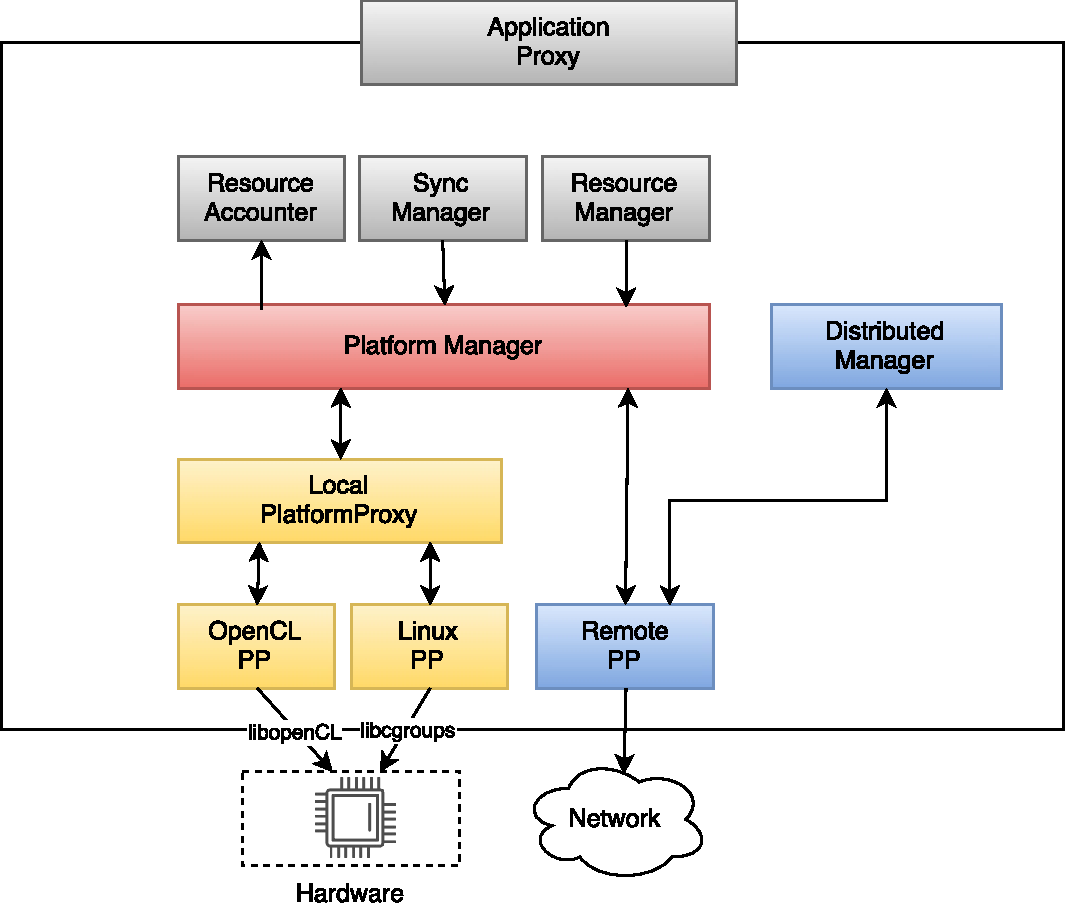
\includegraphics[scale=0.6]{img/cap5-conc-diag.pdf}}
    \caption[BarbequeRTRM distributed components]{The conceptual diagram of BarbequeRTRM distributed components.}
    \label{fig:cap5-conc-diag}
\end{figure}

The \texttt{PlatformManager} class has been also added in order to abstract the
previously described underlying classes with respect to other BarbequeRTRM
components.

\section{DistRib policy}
\label{sec:distribpolicy}
The \textbf{DistRib} policy implemented in BarbequeRTRM is based on a
\textbf{Integer Linear Programming (ILP)} solver. Since the main objective of
this thesis is not to find an advanced policy, but to implement a first exploitation of the \texttt{mig} framework, a classical ILP is proposed.
The proposed policy provides an optimal solution, but it does not scale efficiently.

\subsection{Optimization problem}
The goal of the ILP problem is to find a performance-optimal mapping between
systems and
applications. Please note that this mapping is not necessarily one-to-one: a 
system may have more than one applications running and an application may run
on a different systems. The latter situation is more typical due to the nature
of HPC applications.

Mapping the application onto different systems introduce a significant
overhead due to the network communications between different nodes. Even if
InfiniBand is considered, the intra-host communication with shared memory is
certainly faster \cite{graham2005open}.
In addition to this overhead, heterogeneous systems may
have different performance that must be taken in account. 

Another cost contribution that we can consider in the resource allocation or scheduling policy outcome is the \textbf{oversubscription}:

\begin{PolicyDef}
   An \textbf{oversubscribed} system is a system where the number of
   assigned MPI processes is greater than the number of available processing
   cores (or elements).  
\end{PolicyDef}

This cost may have a strong impact on performance and Open MPI must be therefore aware of oversubscription.

According to Open MPI implementation, for each MPI
process usually
100\% of CPU core is reserved, even if not really used, in order to speed-up the communication
performance. The idea is to avoid as much as possible the overhead due 
to the context switches performed by the operating system. However, this technique produces very bad effects in case of
an oversubscribed system, especially if Open MPI is not aware of oversubscription. We do not delve deeper into the analysis of
oversubscription, since our resource manager does never oversubscribe systems.

Therefore, the cost of oversubscription is proposed in subsequent optimization
problem for completeness, but at present not implemented in the policy.

The ILP formulation proposed is:

\begin{equation}
\min \sum_{a\in A} \sum_{s \in S} \left[ {p_a \cdot ( C^{\text{sys}}(a,s) + C^{\text{dist}}(a,s) +
C^{\text{os}}(a,s) )} \right]
\label{eq:policy_optimization}
\end{equation}

where \(A\) is the set of all applications to be scheduled and \(S\) is the set of all available systems.

Let for each application \(a\):
\begin{itemize}
\item \(\pi(a,s)\):  an integer positive variable that identifies the number of
processes of application \(a\) assigned to system \( s \);
\item \(\phi(a,s)\): a binary variable that values 1 if the application \(a\)
                     is assigned to system \(s\), 0 otherwise;
\item \(p_a\): the priority of the application \(a \);
\item \(r_s\): the penalty to use the system \(s\) (see later for details); 
\item \(K_d\): a constant used as weight coefficient.
\end{itemize}


The variables are \(\pi\) and \(\phi\), the parameters are \(p_a\) and \(r_s\)
and the only constant is \(K_d\).

Obviously, \(\pi\) and \(\phi\) are related and \( \phi \) can be written as:
\[
    \phi(a,s) =  
\begin{cases} 
  1, & \mbox{if } \pi(a,s) > 0 \\ 
  0, & \mbox{ else}
\end{cases}
\]

\begin{equation}
C^{\text{sys}}(a,s) =  r_s \cdot \pi(a,s)
\label{eq:policy_penalty_system}
\end{equation}

\begin{equation}
C^{\text{dist}}(a,s) = K_d \cdot \phi(a,s)
\label{eq:policy_penalty_dist}
\end{equation}

The \(r_s\) penalty is useful when the systems are heterogeneous from the
point of view of the delivered performance: slower systems
may have a high value of \(b_s\), faster system a lower one. If the systems are
homogeneous, \(r_s\) can be set to \(0\) and consequently
\(C^{\text{sys}} = 0\quad \forall a,s\).

In our implementation, the term \(C^{\text{os}}\) is not currently present.
This limitation is not really significant in HPC environments, since a
system oversubscription generally leads to a dramatically drop of performance.

The formulation of the optimization problem in GNU MathProg is presented in
Appendix \ref{app:distrib-ilp-formulation}.

\subsection{The selection algorithm}
The ILP problem may not be feasible, so the solver would not be
able to find a valid solution.
The typical case is when the number of cores requested by all applications is
greater than the available ones. To overcome to this problem, this algorithm
is implemented:
\begin{enumerate}
\item Fill the system and the application vectors with all available resources and ready applications;
\item Try to solve the ILP problem;
\item If OK, enforces the solution;
\item If FAIL, remove the application with less priority and return to (2).
\end{enumerate}

Obviously, the \textbf{starvation} of applications with less priorities
may occur. In order to address this issue we implemented an \emph{aging scheduling}. Every time that an application is
deselected from the scheduling vector its priority is increased. Therefore,
next time the policy runs the non-scheduled applications have higher
probability to be scheduled.
